\chapter{Preliminares}


% https://it.wikipedia.org/wiki/Isosuperficie#cite_note-:2-3
\section{Funciones de distancia con signo}

Una función de distancia con signo (\textit{FDS}) se trata de una aplicación \(f: \mathbb{R}^n\longrightarrow \mathbb{R}\). Esta aplicación transforma un punto en un espacio multidimensional en una distancia con signo a la superficie más cercana. El signo da información sobre cuán cerca/dentro está de los objetos.\\\\
Vamos a simplificar esta clase de funciones multidimensionales en dos casos que podremos adaptar a nuestra computadora. Especialmente, la 2-dimensional y 3-dimensional.\\\\
Como su nombre indica, son funciones que devuelven una distancia signada, un número real. En el caso de las funciones bidimensionales, nos devolverá la distancia mínima a una curva. Mientras que para las funciones tridimensionales, obtendremos la distancia mínima a la superficie. 
\[f(x, y)=d \text{ y } f(x,y,z)=d , d \in \mathbb{R}\text{, respectivamente.}\]
El signo de esta distancia contiene información sobre la escena. Si la distancia es positiva, nos encontramos en el exterior de una figura. Cuando esta es cero, nos encontraremos en la superficie (corteza). Por último, si la distancia es negativa, estaremos dentro de la figura.\\\\
Cuando tratamos de una \textit{superficie o curva cerrada}, según la dimensión, la distancia es negativa. La distancia en positivo representa la profundidad del punto respecto de la corteza. 

\begin{definition}
	Sea \(f(x, y)\) una función de distancia con signo bidimensional, definimos como \textit{isoperímetro} \(L\) al conjunto de puntos tales que \(f(x,y) = 0\).
\end{definition}

\begin{definition}
	Sea \(f(x, y, z)\) una función de distancia con signo tridimensional, definimos como \textit{isosuperficie} \(S\) al conjunto de puntos tales que \(f(x, y, z) = 0\).
\end{definition}
Utilizaremos las coordenadas de los píxeles de nuestra pantalla para pintar una escena bidimensional. Si el valor de la función sobre la coordenada es inferior o igual a cero, le daremos un color, ya que estamos en el interior del \textit{isoperimetro}. \\\\
Para dibujar una escena tri-dimensionales sobre nuestra pantalla plana necesitaremos un \textit{Raymarcher}. Consiste en lanzar un rayo (vector) de módulo incremental hasta aproximarnos a la \textit{isosuperficie}. 
\newpage
\section{La normal de una isosuperficie}

La normal de una superficie es fundamental para la confección de una escena. Especialmente en el modelo de iluminación, que veremos más adelante.

\begin{theorem}
	El vector gradiente \(\nabla f(x_0, y_0, z_0)\)  es ortogonal a la \textit{isosuperficies} \(S\) en el punto \((x_0, y_0, z_0)\)\footnote{Véase la demostración en el libro ""}.
\end{theorem}
% Nota pie, 
En realidad nos quiere decir que la normal de una \textit{isosuperficie} se puede calcular mediante el gradiente, o lo que es lo mismo, el gradiente es la normal de una \textit{isosuperficie}.\\\\
Su demostración está basada en el concepto del plano tangente.\\\\
% https://tutorial.math.lamar.edu/classes/calciii/gradientvectortangentplane.aspx
Veamos cómo podemos calcular el gradiente, por definición:
\[ \nabla f(x, y, z)= < \partial_x f, \partial_y f, \partial_z f, > \]
donde 
\[ \partial_{x_i}f=\lim_{\epsilon\longrightarrow 0}\dfrac{f(x_0,\cdots,x_i+\epsilon,\cdots,x_n)-f(x_0, \cdots, x_n)}{\epsilon} \]
Se puede aproximar computacionalmente, haciendo \(\epsilon = 0.001\).
Finalmente, definimos el gradiente computado como:
\[
\Vec{n}=\nabla f(x, y, z)\approx
\stretchleftright[1000]{\langle}
{\begin{array}{c}
\dfrac{f(x+0.001,y,z)-f(x,y,z)}{0.001}\\
\dfrac{f(x,y+0.001,z)-f(x,y,z)}{0.001}\\
\dfrac{f(x,y,z+0.001)-f(x,y,z)}{0.001} \end{array}}
{\rangle}
\]

\section{Homeomorfismos sobre [0, 1]}

Vamos a definir una aplicación que nos ayudará a deformar funciones de manera continua. Esta aplicación nos será muy útil para manipular las propiedades de la escena, por ejemplo, la intensidad lumínica en nuestro modelo de iluminación, transformación de color, velocidad de un objeto de un punto a otro, etc.

\begin{definition}
    Sea una función \(f:X\longrightarrow Y\), se trata de un homeomorfismo\footnote{Véase la demostración en el libro ""} si,
    \begin{enumerate}
        \item \(f\) es continua.
        \item \(f\) es biyectiva.
        \item \(f^{-1}\) es continua.
    \end{enumerate}
\end{definition}
Restringimos los homeomorfismos a \(X=Y=[0,1]\) con \(f(0)=0\) y \(f(1)=1\). Esta restricción es importante para valores normalizados, ya que aseguramos que sus extremos quedan invariantes.\\\\
Supongamos una imagen en escala de grises con un único canal (para simplificar el ejemplo). El canal acepta un intervalo real \([0, 1]\), donde el color negro es el \(0\) y el blanco, el \(1\).
Además, vamos a definir nuestro \textit{homeomorfismo}, tal que:
\[f(x)=x^8, x \in [0, 1]\]
Así, podemos comprobar que esta función cumple con las propiedades descritas anteriormente. Veamos la forma de los polinómios mónicos hasta el grado \(11\), en \textcolor{blue}{azul} el de grado \(8\).
\begin{figure}[H]
    \centering
    \captionsetup{justification=centering}%,margin=2cm
    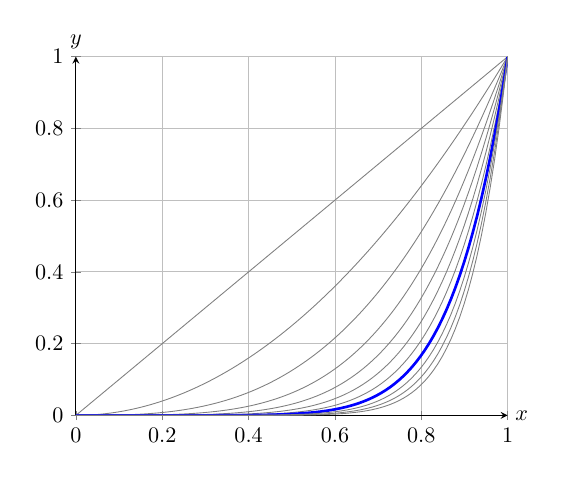
\begin{tikzpicture}[scale=0.8]
        \begin{axis}[
            % Function Properties
            domain=0:1,
            samples=100,
            % Grid Properties
            grid=both,
            % X, Y Coordinates
            axis lines=left,
            compat=newest,
            xlabel=$x$, xlabel style={at={(1,0)}, anchor=west},
            ylabel=$y$, ylabel style={rotate=-90,at={(0,1)}, anchor=south}
        ]
            \addplot[gray] (x,x);
            \addplot[gray] (x,x^2);
            \addplot[gray] (x,x^3);
            \addplot[gray] (x,x^4);
            \addplot[gray] (x,x^5);
            \addplot[gray] (x,x^6);
            \addplot[gray] (x,x^7);
            \addplot[blue, very thick] (x,x^8);
            \addplot[gray] (x,x^9);
            \addplot[gray] (x,x^10);
            \addplot[gray] (x,x^11);
        \end{axis}
    \end{tikzpicture}
    \caption{Polinomios mónicos hasta grado 11} \label{fig:M1}
\end{figure}

Vemos que los valores inferiores a \(0.6\) se transforman a valores próximos a \(0.0\), oscureciendo los tonos grises. Mientras que los colores más claros, se mantienen.
\begin{figure}[H]
  \centering
  \captionsetup{justification=centering}%,margin=2cm
  \subfloat[Imagen original]{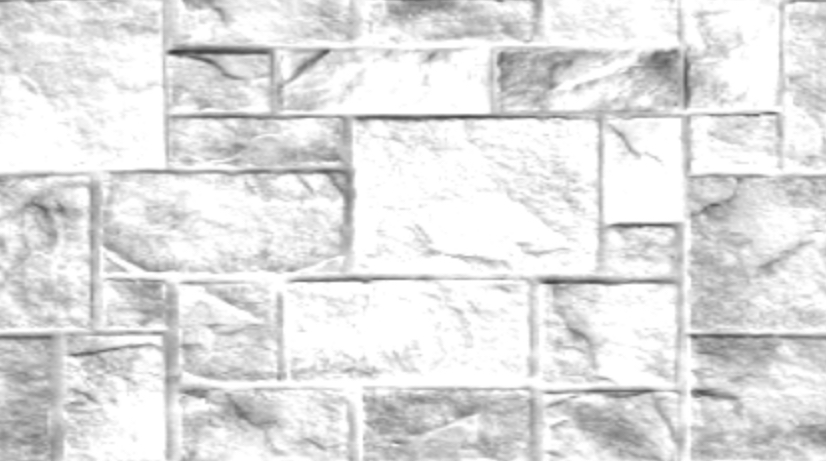
\includegraphics[width=0.4\textwidth]{secciones/imagenes/pol8-img-left.jpeg}\label{fig:white}}
  \hfill
  \subfloat[\(f\) aplicada sobre la imagen original]{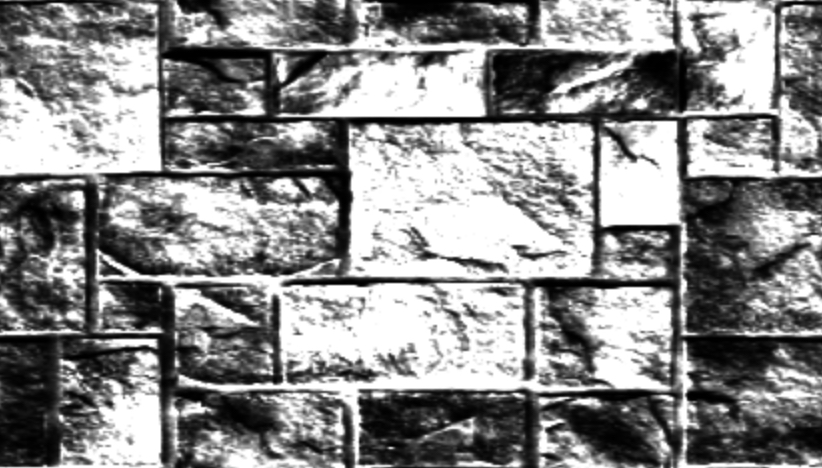
\includegraphics[width=0.4\textwidth]{secciones/imagenes/pol8-img-right.jpeg}\label{fig:black}}
  \caption{Aplicación de un homeomorfismo a una imagen de grises.}
\end{figure}
% Pie Define monico
En el ejemplo anterior hemos visto un polinomio mónico\footnote{La definición de mónico se puede encontrar en el libro ""}, pero podemos utilizar cualquier otra función que cumpla con las restricciones. Aún así, es recomendable utilizar polinomios debido a la baja necesidad computacional y capacidad de aproximar cualquier función utilizando el \textit{Polinomio de Taylor}\footnote{Aproximando funciones utilizando polinomios}, por ejemplo:
\[ f(x)=\sin\left(\dfrac{\pi}{2}x\right)\approx \max\left(\dfrac{\pi}{2}x-\dfrac{\pi^3}{48}x^3+\dfrac{\pi^5}{3840}x^5, 1\right) \]

\section{Homotopías e interpolaciones.}
% Nota pie
En esta última sección, vamos a ver una aplicación matemática que es utilizada para animación y texturización.
Como hemos visto antes, vamos a centrarnos en el intervalo \([0, 1]\). Podemos trabajar con cualquier intervalo, pero antes deberemos normalizar y finalmente, reescalar.

\begin{definition}
    Dadas dos aplicaciones \(f, g:X\longrightarrow Y\), continuas, decimos que son homotópicas\footnote{Definición de homotopía}. Si existe una aplicación \(H\), también continua, tal que:
    \[ H:X\times[0,1]\longrightarrow Y \]
    \[ H(x, 0)=f(x) \]
    \[ H(x, 1)=g(x) \]
\end{definition}
% nota pie
\begin{definition}
    Dada una homotopía \(H\), llamaremos función de interpolación lineal o función de mezcla con peso\footnote{Encontramos este término en libros como} a la apliación:
    \[H(x, t)=(1-t)\cdot f(x) + t\cdot g(x)\]
\end{definition}
Como podemos observar,  la última definición es una homotopía, ya que, la suma de dos funciones continiuas es siempre continua y los extremos resultan \(f(x)\) y \(g(x)\), respectivamente.\\\\
Como sabemos, \(t\in[0,1]\), por lo que podemos aplicar un \textit{homomorfismo} \(p(x)\) y tener así, una versión más general.
    \[H(x, t)=(1-p(t))\cdot f(x) + p(t)\cdot g(x)\]
Veamos un ejemplo, supongamos que \(f(x)\) y \(g(x)\) son los colores de una imagen 3-canal y como \(t\), una tercera imagen con un canal \([0,1]\), que actuará como máscara.
\begin{figure}[H]
  \centering
  \captionsetup{justification=centering}%,margin=2cm
  \subfloat[Imagen \(f(x)\)]{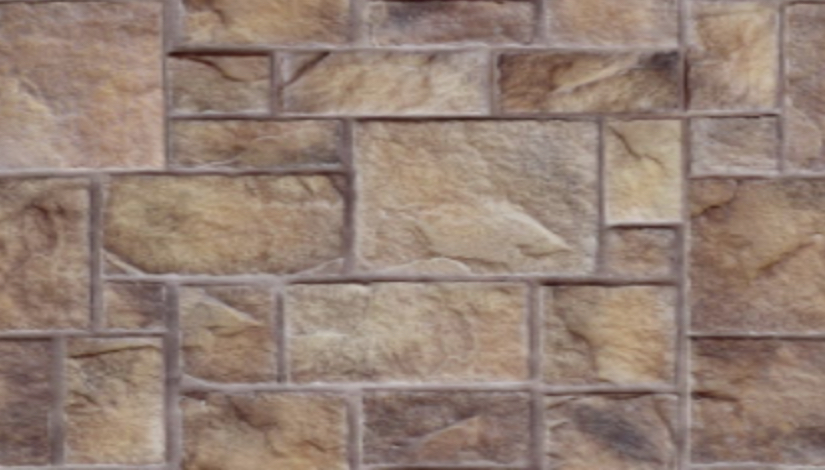
\includegraphics[width=0.33\textwidth]{secciones/imagenes/texture-wall.jpeg}\label{fig:left}}
  \subfloat[Imagen \(g(x)\)]{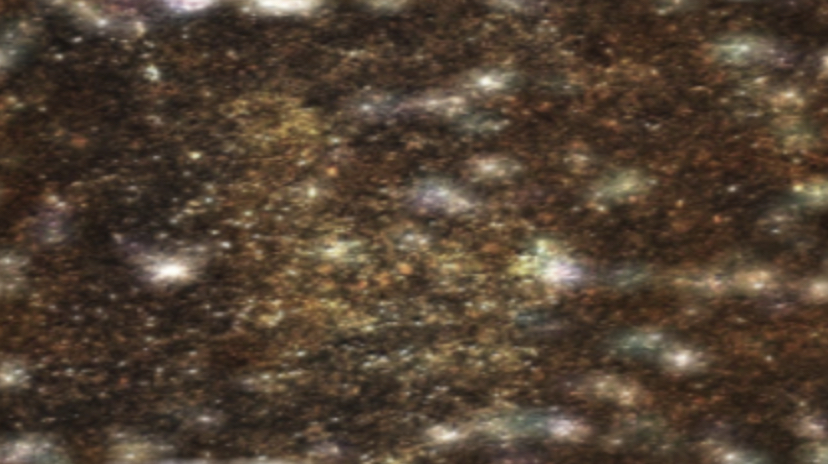
\includegraphics[width=0.33\textwidth]{secciones/imagenes/texture-galaxy.jpeg}\label{fig:right}}
  \subfloat[Máscara \(t\)]{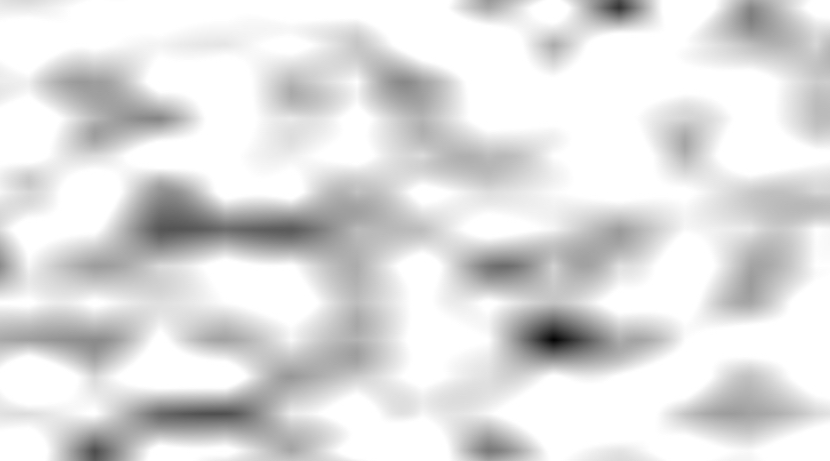
\includegraphics[width=0.33\textwidth]{secciones/imagenes/mask.jpeg}\label{fig:result}}
  \caption{Imagen \(f(x)\), Imagen \(g(x)\) y Máscara \(t\)}
\end{figure}
Veamos los resultados obtenidos utilizando diferentes homomorfismos.
\begin{figure}[H]
  \centering
  \captionsetup{justification=centering}%,margin=2cm
  \subfloat[Interpolación con el homomorfismo \(p(t)=t\)]{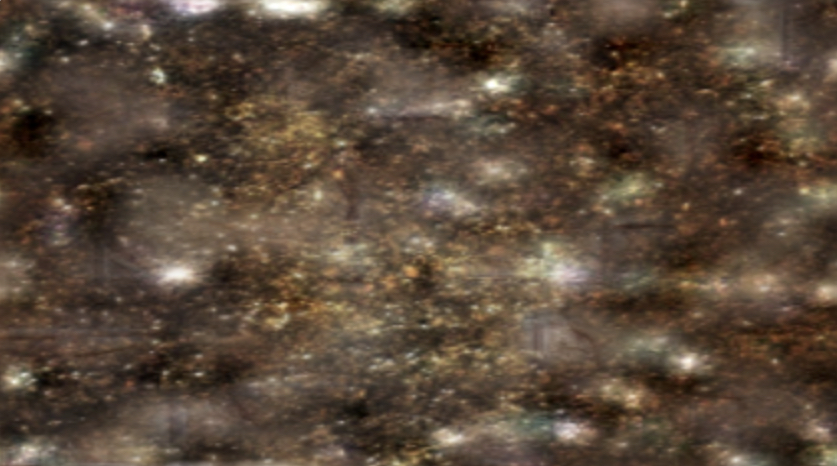
\includegraphics[width=0.4\textwidth]{secciones/imagenes/masking-result-1.jpeg}\label{fig:result1}}
  \hfill
  \subfloat[Interpolación con el homomorfismo \(p(t)=t^4\)]{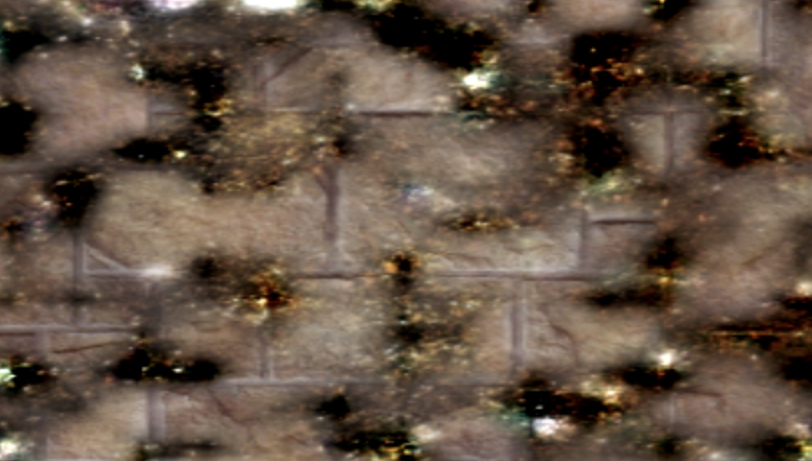
\includegraphics[width=0.4\textwidth]{secciones/imagenes/masking-result-2.jpeg}\label{fig:result2}}
  \caption{Interpolaciones con distintos homomorfismos.}
\end{figure}
